% ══════════════════════════════════════════════════════════════════════════════
%  CAPITOLO — MODELLI DI REGRESSIONE PER CONTEGGI
%  Etichette: ch:glm, sec:glm_unit, sec:glm_spec, sec:glm_overdisp,
%             sec:glm_effects, sec:glm_time, sec:glm_holdout, sec:glm_summary
% ══════════════════════════════════════════════════════════════════════════════

\chapter{Modelli di Regressione per Conteggi}
\label{ch:glm}
Si introducono ora alcuni dei modelli statistici utilizzati per spiegare la 
frequenza di donazione dei singoli donatori, per poi commentare i risultati di
tale analisi. La domanda a cui si cercherà di rispondere è:
``che comportamento assume il singolo donatore? Quali sono
le probabilità che torni a donare?''. La domanda è di tipo inferenziale: a
parità di ogni altra condizione, quali caratteristiche sono associate a una
frequenza di donazione più alta? Quanto esse influiscono sulla frequenza stessa?

La risposta è un conteggio: questa caratteristica di per sé pone un vincolo
sulla classe di modelli che sarà possibile utilizzare.
La regressione lineare ordinaria è inadeguata: nei conteggi la varianza cresce con
la media, mentre in questi tipi di modelli essa è assunta costante.
Si ricorre quindi ai modelli lineari generalizzati per dati di
conteggio~\cite{CameronTrivedi2013}, nelle versioni di Poisson e binomiale
negativa, confrontate nella \cref{sec:glm_overdisp}.

% ───────────────────────────────────────────────────────────────────────
\section{Unità di analisi e variabile risposta}
\label{sec:glm_unit}

La scelta dell'unità di osservazione
determina cosa il modello può vedere. Dopo aver passato al vaglio le possibilità,
se ne sono escluse alcune apparentemente intuitive per le seguenti motivazioni:

\paragraph{Riga evento: }
Il dataset originale è composto riga per evento di donazione; tra le colonne,
è presente \texttt{num\_don}, aggregato di livello
superiore: esso rappresenta il numero di donazioni del gruppo (donatore $\times$ anno $\times$
tipologia) cui la riga appartiene, uguale per ogni riga appartenente a quel gruppo
(\cref{sec:dataset}). Se si stimasse un modello a partire da quelle righe e con \texttt{num\_don}
come variabile risposta, ogni gruppo entra nella verosimiglianza tante volte quante sono
le sue donazioni: più grande è il singolo gruppo e più peso avrà, proporzionalmente
al valore della variabile risposta. La media stimata è quindi distorta, e di conseguenza
anche gli errori standard e ogni test di dispersione. 
% La differenza è misurabile: la media della risposta calcolata
%sulle righe è $2{,}47$, quella calcolata sui gruppi $1{,}70$.

\paragraph{Deduplicazione.}
Una correzione del fenomeno appena descritto è la \textbf{deduplicazione}, ovvero
mantenere una sola riga per gruppo (donatore $\times$ anno $\times$ tipologia).
Ciò fa però insorgere due ulteriori problemi.

Il primo, in ordine di importanza, è che \textbf{la risposta é troncata}: una tripla
esiste solo se quella donazione c'è stata, mentre l'informazione riguardante
gli anni in cui il donatore è rimasto in attivo viene persa. Il modello é
\textbf{cieco} circa l'evento che il \cref{ch:retention} ha mostrato essere il più
frequente di tutti: l'abbandono. E la diagnosi di dispersione ne risente in
modo sostanziale: misurato sui soli anni attivi, il rapporto varianza/media è
$\mathbf{1{,}23}$ (quasi equidispersione); considerando anche gli anni di
inattività,essa diventa $\mathbf{2{,}45}$.

Il secondo è che le osservazioni restano \textbf{raggruppate per donatore}: lo
stesso soggetto compare in molti anni, e le sue osservazioni \textbf{non} sono
indipendenti. Deduplicare elimina la replicazione dentro il gruppo, ma non
questa seconda fonte di dipendenza, che va trattata a parte (si veda il
paragrafo sugli errori standard nella \cref{sec:glm_spec}).

\paragraph{Il grano adottato.}
La risposta è il \textbf{numero di donazioni per donatore e anno, con gli anni
a zero materializzati}: il panel costruito al terzo e ultimo stadio della pipeline
(\cref{sec:cleaning}), composto da \textbf{514\,098 righe}, il $63{,}9\%$ delle quali a
zero. Il campione di stima va dal 2013 in poi
(\textbf{444\,240 righe}, 43\,298 donatori), essendoci incertezza sulla storia dei donatori
nei primi anni osservati (tutti sono considerati "esordienti" nel 2009, primo anno a disposizione).

Così facendo, \textbf{la somma della
risposta su un anno è il totale di quell'anno}. Il modello individuale di
questo capitolo e la previsione aggregata dell'\cref{ch:forecast} misurano
quindi la stessa grandezza e non possono contraddirsi.

% ───────────────────────────────────────────────────────────────────────
\section{Modello GLM per conteggi}
\label{sec:glm_model}
Prima di discutere il modello usato nelle previsioni svolte, si introduce il concetto di
GLM~\cite{McCullaghNelder1989}.

Un \textbf{GLM} (Generalized Linear Model) è un modello statistico definito
da tre componenti principali: 
\begin{itemize}
    \item \textbf{Componente casuale}: com'è distribuita la variabile risposta $\mathbf{Y}$ appartenente
    alla famiglia esponenziale; 
    \item \textbf{Predittore lineare}: costruito nella forma 
    $\eta = \beta_{0} + \beta_{1}x_{1} + \beta_{2}x_{2} + ... + \beta_{n}x_{n}$;
    \item \textbf{Funzione di legame}: collega la media della risposta al predittore: 
    $g(\mu) = \eta,  \mu = \mathbb{E}[\mathbf{Y}]$.
\end{itemize}

\paragraph{GLM di Poisson.} Durante lo studio si è ipotizzato l'utilizzo della \textbf{GLM di Poisson} 
--- essa ha un solo parametro $\lambda$ e si ha:
\begin{equation}
    \mathbb{E}[\mathbf{Y}] = \mathbb{V}[\mathbf{Y}] = \lambda
\end{equation}

Analizzando i dati, si nota come $\mathbb{V}[\mathbf{Y}] \gg \mathbb{E}[\mathbf{Y}]$ (\textbf{sovradispersione}); 
la GLM di Poisson è stata quindi considerata inadatta a descrivere il fenomeno osservato.

\paragraph{GLM Binomiale Negativa.} La \textbf{GLM Binomiale Negativa} è stata quindi
considerata come alternativa; intuitivamente, essa può essere vista come una
\textbf{Poisson}, dove la singola osservazione $i$ ha un proprio \textbf{tasso latente}
$\mu_i u_i$, $u_i$ \textbf{fattore di eterogeneità non osservata} diverso per ogni soggetto,
distribuito secondo una \textbf{Gamma} di media 
$1$ e varianza $\alpha$.
Si ha quindi:
\begin{equation}
    \mathbf{Y}_{i} | u_{i} \sim \text{Po}(\mu_{i}u_{i}), \quad u_{i} \sim \Gamma(1/\alpha, \alpha)
\end{equation}
Integrando per il fattore di eterogeneità $u_i$, si ha:
\begin{equation}
    \mathbb{E}[\mathbf{Y}_{i}] = \mu_{i}, \quad \mathbb{V}[\mathbf{Y}_{i}] = \mu_{i} + \alpha\mu_{i}^{2}
    \implies \mathbf{Y}_{i} \sim \text{NB}(\mu_{i}, \alpha) 
\end{equation}

Questa \textit{parametrizzazione} è detta \textbf{NB2}. $\alpha$ misura la \textbf{sovradispersione} del modello:
se $\alpha=0$, si collassa nella \textbf{Poisson} (caso limite).

\paragraph{Link e forma del modello.} Il terzo elemento della specifica è la
\textbf{funzione di legame}, che in questo caso è il \textbf{logaritmo naturale}:
\begin{equation}
    \ln\mu_i = \ln\mathbb{E}[\mathbf{Y}_i \mid \mathbf{x}_i] = \mathbf{x}_{i}^\top\boldsymbol{\beta}
\end{equation}

Questa scelta è motivata dal fatto che la risposta è un conteggio, quindi non può assumere valori negativi;
il modello avrà quindi la stessa forma della media di un GLM di Poisson, ma con una varianza più flessibile: 
ciò lo rende più fedele e adatto ai dati osservati che presentano la sovradispersione discussa in precedenza.

\paragraph{Stima dei parametri.}
Solitamente la stima dei parametri $\beta$ e $\alpha$ avviene tramite il 
\textbf{metodo della massima verosimiglianza} (MLE).

$\alpha$ può essere stimato anche con il \textbf{metodo dei momenti}: si stima
prima il modello di Poisson, che fornisce le medie $\hat{\mu}_i$, e si sceglie
$\alpha$ in modo che la relazione $\mathbb{V}[Y_i] = \mu_i + \alpha\mu_i^2$ valga
in media sui residui,
\begin{equation}
    \hat{\alpha} = \frac{1}{n}\sum_{i=1}^{n}
    \frac{(y_i - \hat{\mu}_i)^2 - \hat{\mu}_i}{\hat{\mu}_i^2}.
\end{equation}
Nel modello utilizzato nelle analisi $\alpha$ è stato stimato con quest'ultimo
metodo e poi fissato come costante: $\hat{\alpha} = 2{,}37$.
% ───────────────────────────────────────────────────────────────────────

\section{Specificazione}
\label{sec:glm_spec}

Il modello ha forma
\begin{equation}
    \log \mathbb{E}[Y_{it} \mid \mathbf{x}_{it}]
    = \beta_0
    + \beta_{\text{a}}\,\text{età}_{it}
    + \beta_{\text{c}}\,\text{carriera}_{it}
    + \beta_{\ell}\,\text{troncato}_{i}
    + \boldsymbol{\gamma}^\top \mathbf{d}_{it}
    + \delta\,(\text{anno}_t - 2016),
    \label{eq:glm_form}
\end{equation}
dove $i$ indicizza il donatore e $t$ l'anno, e $\mathbf{d}_{it}$ raccoglie le
variabili categoriche. Con legame logaritmico ogni coefficiente esponenziato si
interpreta come \emph{Incidence Rate Ratio} (IRR): il rapporto fra il numero
atteso di donazioni con e senza la caratteristica, tenute ferme le altre.

Si pone particolare attenzione ad alcune scelte di specifica:

\paragraph{Carriera.}
La variabile \texttt{carriera} è il numero di anni trascorsi dall'inizio
dell'attività donazionale, misurato sulla data di inizio attività registrata
nel dato grezzo (\texttt{first\_activity\_date}) e, dove questa manca, sul primo
anno osservato. Misurarla dal primo anno osservato farebbe sembrare esordienti
i donatori già attivi prima del 2009. La variabile \texttt{troncato} marca i
donatori la cui carriera risulta iniziata prima del loro primo anno osservato:
per loro la storia donazionale precedente (tipologia, frequenza) non è nel
dataset, anche se l'anzianità è nota.

Senza il controllo per la carriera, un'eventuale coorte di ingresso ne
assorbirebbe l'effetto. Nella variante che aggiunge la coorte quinquennale di
ingresso le coorti recenti hanno IRR crescenti, fino a $3{,}5$ per quella del
2025 e fino a $4{,}0$
se si toglie anche la carriera. Misurano il fatto che quei donatori sono osservati soltanto nei loro primi
anni, che sono quelli con maggiore attività.

\paragraph{Categorie di riferimento esplicite.}
Le categorie di riferimento sono imposte, non ereditate dall'ordinamento
alfabetico: \textbf{P} (periodico) per la classe donatore e \textbf{SANGUE} per
la tipologia, cioè le categorie modali. Ogni IRR si legge così come confronto
con il donatore tipico, e l'intervallo di confidenza è calcolato rispetto a una
base ampia. Le categorie rare della classe donatore (la classe A compare una
volta sola in diciassette anni) non entrano nel campione di stima.

\paragraph{Tipologia ritardata agli anni precedenti.}
Al grano donatore-anno la tipologia dell'anno corrente è un attributo della
risposta: entra quindi la tipologia \emph{prevalente negli anni
precedenti}, che è causale per costruzione.

\paragraph{Una specifica non identificata.}
Un limite strutturale fondamentale è il seguente:
\textbf{età, periodo e coorte di ingresso non sono identificabili insieme}, 
perché anno $=$ anno di ingresso $+$ anni di carriera. Una specifica
che li contenga tutti e tre stima coefficienti identificati soltanto dalla
forma funzionale imposta, come il quinquennio usato come coorte, e non dai dati
stessi. Il modello principale che viene usato
esclude quindi la coorte come cooefficiente.

\paragraph{Errori standard.}
Tutti gli errori standard riportati sono \textbf{robusti per cluster di
donatore}: non c'è assunzione di indipendenza tra entry dello stesso soggetto
in anni differenti.

% ───────────────────────────────────────────────────────────────────────
\section{Sovradispersione e scelta della distribuzione}
\label{sec:glm_overdisp}

Il modello facente uso della distribuzione di Poisson impone 
$\mathbb{E}[Y] = \mathrm{Var}[Y]$. Sul panel
completo, la risposta ha media $0{,}69$ $\neq$ varianza $1{,}68$, con
varianza/media $\mathbf{2{,}45}$: è evidente la sovradispersione del modello.

Il modello binomiale negativo non ha vincoli, in quanto introduce un parametro di
dispersione $\alpha$:
\begin{equation}
    \mathrm{Var}[Y] = \mu + \alpha\,\mu^2 .
    \label{eq:nb_var}
\end{equation}
Come anticipato nella \cref{sec:glm_model}, la stima ottenuta tramite il metodo dei momenti
è $\hat{\alpha} = 2{,}37 \gg 0$.
Questo valore, anziché venire ristimato, entra nel
modello come costante. Di conseguenza i due
modelli hanno lo stesso numero di parametri e la binomiale negativa non
subisce una penalizzazione per il parametro $\alpha$; con una differenza di AIC di sei cifre il punto è
irrilevante per la conclusione, ma va detto. Il confronto sui criteri di informazione
(\cref{tab:glm_fit}) è netto: la differenza di AIC è di \textbf{115\,936 punti}
a favore del modello binomiale negativo.

\begin{table}[ht]
\centering
\caption{Adattamento dei due modelli sul panel donatore-anno (444\,240
osservazioni).}
\label{tab:glm_fit}
\begin{tabular}{@{}lrrr@{}}
\toprule
\textbf{Modello} & \textbf{AIC} & \textbf{BIC} & \textbf{Log-veros.} \\
\midrule
Poisson                   & 986\,075{,}9 & 986\,196{,}9 & $-493\,026{,}9$ \\
Binomiale negativo        & \textbf{870\,140{,}3} & \textbf{870\,261{,}3} & $\mathbf{-435\,059{,}1}$ \\
\midrule
Differenza                & $115\,935{,}6$ & $115\,935{,}6$ & $57\,967{,}8$ \\
\bottomrule
\end{tabular}
\end{table}

Su una tabella deduplicata e ristretta a una singola annualità, quindi,
la binomiale negativa collassa
sulla Poisson, e la sovradispersione sembra svanire  (\cref{sec:dash_overdisp}). La verifica appena svolta
mostra che quell'esito era un artefatto del troncamento: osservando i soli anni attivi,
si osserva una popolazione già selezionata, a cui sono già stati rimossi gli zeri.
Con gli zeri al loro posto, la sovradispersione è massiccia e la scelta della
binomiale negativa non è in discussione.

Tutti i risultati che seguono si riferiscono al modello binomiale negativo.

% ───────────────────────────────────────────────────────────────────────
\section{Effetti stimati}
\label{sec:glm_effects}

\begin{table}[ht]
\centering
\caption{Modello binomiale negativo al grano donatore-anno: IRR, intervalli di
confidenza al 95\% con errori standard robusti per cluster di donatore, e
$p$-value. È omesso il livello residuale \textsc{altro} della tipologia
pregressa, troppo raro per essere stimato con precisione (IRR $0{,}78$,
$p = 0{,}61$).}
\label{tab:glm_irr}
\begin{tabular}{@{}lrrl@{}}
\toprule
\textbf{Termine} & \textbf{IRR} & \textbf{IC 95\%} & \textbf{$p$} \\
\midrule
\multicolumn{4}{@{}l}{\emph{Caratteristiche del donatore}} \\
Genere F (rif.\ M)          & $\mathbf{0{,}585}$ & $[0{,}566;\ 0{,}605]$ & $<0{,}001$ \\
Età (per anno)              & $1{,}0007$ & $[0{,}9994;\ 1{,}0020]$ & $0{,}31$ \\
Anni di carriera (per anno) & $0{,}980$  & $[0{,}977;\ 0{,}983]$ & $<0{,}001$ \\
Carriera troncata a sinistra& $0{,}907$  & $[0{,}866;\ 0{,}951]$ & $<0{,}001$ \\
\addlinespace
\multicolumn{4}{@{}l}{\emph{Classe donatore all'ingresso} (rif.\ P --- periodico)} \\
D --- prima donazione       & $0{,}786$  & $[0{,}751;\ 0{,}821]$ & $<0{,}001$ \\
O --- occasionale           & $0{,}490$  & $[0{,}470;\ 0{,}512]$ & $<0{,}001$ \\
\addlinespace
\multicolumn{4}{@{}l}{\emph{Tipologia prevalente pregressa} (rif.\ SANGUE)} \\
AFPLTPLASM                  & $2{,}194$  & $[1{,}862;\ 2{,}586]$ & $<0{,}001$ \\
PLASMAF                     & $\mathbf{1{,}766}$ & $[1{,}660;\ 1{,}879]$ & $<0{,}001$ \\
\addlinespace
\multicolumn{4}{@{}l}{\emph{Tempo}} \\
Anno (rispetto al 2016)     & $0{,}941$  & $[0{,}938;\ 0{,}943]$ & $<0{,}001$ \\
\midrule
Dispersione $\hat{\alpha}$  & \multicolumn{3}{l}{$2{,}37$} \\
\bottomrule
\end{tabular}
\end{table}

\paragraph{Genere.}
È l'effetto più netto del modello. A parità di ogni altra condizione, le
donatrici (F) registrano una frequenza attesa inferiore rispetto ai donatori (M),
pari al $\mathbf{58{,}5\%}$ di quella
dei donatori maschi. La motivazione è da ricercare nella normativa italiana~\cite{dm2015},
che impone alle donne in età fertile un intervallo minimo fra donazioni di sangue intero più
lungo e un numero massimo annuo inferiore (due contro quattro), a cui si aggiunge la
maggiore frequenza di sospensioni per anemia. \textbf{É quindi un vincolo regolamentare e normativo},
interpretarlo altrimenti sarebbe un errore sostanziale.

\paragraph{Età e anzianità.}
L'effetto dell'età anagrafica è \textbf{statisticamente indistinguibile da
zero} ($p = 0{,}31$), mentre quello dell'anzianità di carriera è netto e
negativo: $-2\%$ di frequenza attesa per ogni anno trascorso dall'inizio
dell'attività. Poiché l'età è già nel modello, questo calo non può essere
attribuito all'invecchiamento o all'uscita dai limiti di età: riflette il fatto
che il panel tiene ogni donatore anche dopo che ha smesso, e che al crescere
degli anni di carriera cresce la probabilità di averlo già fatto. È, letta al
grano donatore-anno, la stessa perdita progressiva descritta nel
\cref{ch:retention}.

Il risultato sull'età dipende interamente dal controllo per anzianità.
Togliendolo dalla specifica, l'età riemerge con un IRR di $0{,}9963$
($-0{,}4\%$ per anno d'età) e un $p$-value inferiore a $0{,}001$ --- un
effetto apparentemente solido. Senza quel controllo il coefficiente dell'età
sta misurando l'anzianità: a parità di anno, i donatori più anziani hanno in
media carriere più lunghe, quindi più anni trascorsi dall'ingresso e più
probabilità di avere già smesso, e il modello attribuisce all'età ciò che
appartiene alla carriera.

\paragraph{Classe donatore, e una rottura di codifica.}
L'ordinamento stimato è quello atteso (periodico $>$ prima donazione $>$
occasionale): un donatore entrato come occasionale
dona meno della metà di uno entrato come periodico, con intervalli stretti ---
il che, come detto sopra, dipende dall'aver imposto \textbf{P} come
riferimento anziché ereditarlo.

Sulla variabile grava però un problema di fondo: \textbf{la classe donatore
cambia codifica nel 2016}. La classe O passa da circa 3\,000
casi l'anno a una decina fra il 2015 e il 2017, e contemporaneamente compare
la classe D, prima inesistente (\cref{fig:donor_class_regime}).

\begin{figure}[H]
    \centering
    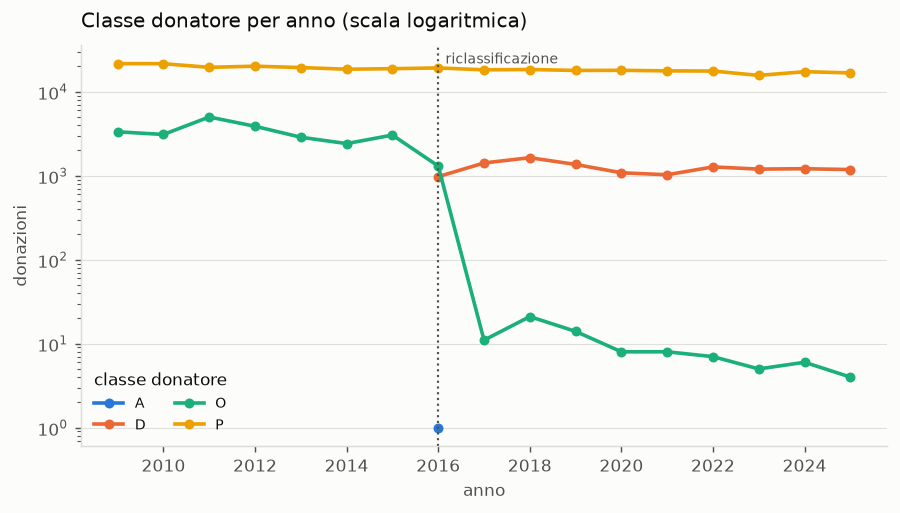
\includegraphics[width=0.9\linewidth]{img/fig_donor_class_regime.png}
    \caption{Donazioni per classe donatore e anno, scala logaritmica. La
    discontinuità del 2016 è una riclassificazione amministrativa.}
    \label{fig:donor_class_regime}
\end{figure}

È una riclassificazione amministrativa.
Nel modello la variabile entra come \emph{classe all'ingresso}, che
attenua il problema ma non lo elimina. L'ordinamento
stimato va quindi letto come robusto nella direzione ma non come una misura
comparabile fra i due regimi, e l'assunzione ``D $=$ prima donazione'' andrebbe
verificata direttamente con il DIMT prima di essere data per buona.

\paragraph{Tipologia di donazione.}
Chi ha donato prevalentemente plasma continua a donare $1{,}77$ volte più
spesso di chi ha donato prevalentemente sangue intero. Ciò é dovuto, come altre
statistiche, ad una questione di regolamentazioni: il plasma è ricostituito in giorni
anziché in settimane, e l'intervallo minimo fra due plasmaferesi è di 14 giorni
contro i 90 del sangue intero~\cite{dm2015}.

% ───────────────────────────────────────────────────────────────────────
\section{Andamento temporale}
\label{sec:glm_time}

Il termine temporale è negativo e netto: a profilo fissato la frequenza attesa
scende del $5{,}9\%$ all'anno (\cref{fig:glm_trend}).

\begin{figure}[H]
    \centering
    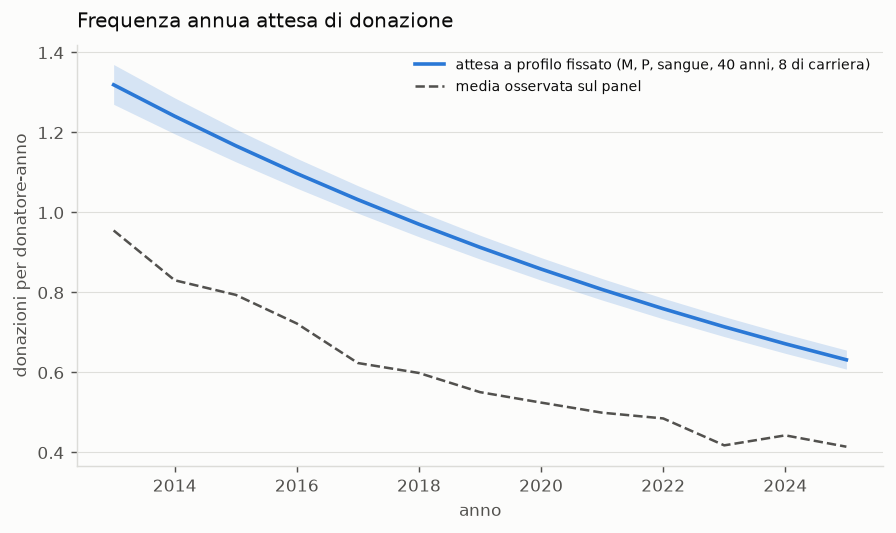
\includegraphics[width=0.95\linewidth]{img/fig_glm_trend.png}
    \caption{Frequenza annua attesa di donazione secondo il modello binomiale
    negativo, a profilo fissato (maschio, classe P, sangue intero, 40 anni,
    otto anni di carriera), con intervallo di confidenza al 95\%; in
    tratteggio, la media osservata sul panel.}
    \label{fig:glm_trend}
\end{figure}

Il valore va letto con attenzione, perché è più ripido del calo aggregato del
\cref{ch:eda} ($-28\%$ in diciassette anni): il panel accumula donatori, compresi gli
occasionali o chi interrompe l'attività di donazione,
quindi la sua composizione si sposta di anno in anno verso i dormienti. La
frequenza media \emph{per riga di panel} cala per questo motivo oltre che per
un'eventuale riduzione di attività dei donatori vivi.

Ciononostante, il risultato sostantivo resta lo stesso:
\textbf{l'intensità individuale attesa non sta crescendo}. Non c'è, nei dati, 
la compensazione da parte dei donatori esistenti
che avrebbe potuto tenere stabile il volume aggregato --- coerentemente con
quanto già osservato nella \cref{sec:intensity}, dove il numero medio di
donazioni per donatore attivo si rivela piatto lungo tutti i diciassette anni.
Quanto questo sia preoccupante dipende anche dalla domanda: se nello stesso
periodo il fabbisogno di emocomponenti del territorio fosse calato, una raccolta
più piccola potrebbe restare adeguata. È una verifica che richiede i dati di
consumo, che questo lavoro non ha.

% ───────────────────────────────────────────────────────────────────────
\section{Verifica predittiva}
\label{sec:glm_holdout}

L'AIC misura l'adattamento in campione e premia il modello più flessibile. Per
una verifica indipendente serve una divisione dei dati, che va
scelta coerentemente all'uso del modello.

Una divisione \emph{casuale} sulle righe non è adeguata qui, per due
ragioni cumulative:
\begin{itemize}
    \item la correlazione: donazioni dello stesso soggetto potrebbero finire
 sia in addestramento che in verifica;
    \item dati \emph{temporali}: le donazioni sono posizionate sulla linea del tempo e,
mischiandole casualmente, una donazione avvenuta nel 2011 potrebbe finire nel test,
mentre una del 2024 nel training set.
\end{itemize}


La verifica corretta è quella temporale: si stima su tutto ciò che precede
un'origine e si valuta su ciò che segue. È il criterio applicato
sistematicamente nell'\cref{ch:forecast}, dove i modelli per donatore di questo
capitolo sono confrontati con gli altri candidati sullo stesso backtest a
origine mobile. L'esito, riportato nella \cref{tab:fc_backtest}, è piuttosto significativo:
\textbf{i modelli per donatore, sommati per ottenere il volume aggregato,
sbagliano circa il doppio del trend smorzato} ($6{,}5\%$ contro $3{,}5\%$ di
MAPE), e la causa è identificata nella \cref{sec:fc_volume}.

Questo non annulla lo studio eseguito, ma ne circoscrive l'utilizzo: il modello appena descritto
serve a \emph{spiegare} la frequenza donazionale e per quello i suoi
coefficienti sono informativi. Non è lo strumento migliore per \emph{prevedere}
il volume aggregato.

% ───────────────────────────────────────────────────────────────────────
\section{Sintesi e limiti}
\label{sec:glm_summary}

\paragraph{1. I vincoli clinici pesano sul comportamento.}
Due degli effetti più forti e più precisi, genere (IRR $0{,}585$) e tipologia
prevalente (IRR $1{,}77$ per la plasmaferesi), misurano in larga parte la
regolamentazione: intervalli minimi fra donazioni e tetti annui differenziati.
Qualunque politica di intensificazione della raccolta deve partire da qui: il
margine di manovra sui donatori esistenti è vincolato in alto da regole
cliniche, non dalla loro disponibilità.

\paragraph{2. L'anzianità di sistema conta, l'età anagrafica no.}
Controllando per gli anni di carriera, l'effetto dell'età anagrafica sparisce
($p = 0{,}31$). Ciò che distingue un donatore assiduo non è quanti anni ha, ma
da quanto tempo dona --- il che rafforza la lettura del \cref{ch:retention}: il
valore di un donatore si costruisce nel tempo, e perderlo presto costa molto
più di quanto suggerisca il conteggio delle donazioni mancate nel primo anno.

\paragraph{Limiti.}
\textbf{Età, periodo e coorte non sono identificabili insieme:} il modello
principale esclude la coorte di ingresso per questo motivo, e la variante che
la include produce coefficienti identificati dalla forma funzionale:
separare effetto di età ed effetto di coorte richiede
un'assunzione esterna che qui non si è voluta imporre. \textbf{Manca una
struttura longitudinale esplicita:} gli errori standard robusti per cluster
tengono conto della correlazione fra anni dello stesso donatore, ma il
modello non stima un effetto individuale, e un modello a effetti casuali sul
donatore sarebbe la specifica più ricca e lo sviluppo naturale di questo
capitolo. Pesa inoltre \textbf{la rottura di codifica di
\texttt{donor\_class}} discussa nella \cref{sec:glm_effects}: la variabile
confronta due schemi amministrativi diversi, e l'ordinamento va letto come
robusto nella direzione ma non nella scala. Infine il modello \textbf{non ha
interazioni}: è puramente additivo e non può cogliere, ad esempio, che il
divario di genere sia diverso fra sangue intero e plasmaferesi, ipotesi
plausibile dato che i tetti normativi differiscono per tipologia.

% ══════════════════════════════════════════════════════════════════════════════
%  Fine Capitolo — Modelli di Regressione per Conteggi
% ══════════════════════════════════════════════════════════════════════════════
